\chapter{Results}
\label{ch:results-en}

This chapter reports observations and registered decisions first; broader
interpretation is deferred to Chapter~\ref{ch:discussion}. Every major block is tied
explicitly to C01--C11 so claim status is not strengthened when a numerical result is
converted into prose.

Results follow the order of the research program. Numerical tables governed by the
thesis data contract are generated in CI from machine-readable summaries. This
separates narrative presentation from manual number transcription while retaining
SHA-256 bindings to tracked source evidence.

\section{Stage 1 and Stage 2: Quality and Computational Cost}
\label{sec:results-stage12-en}

Stage~1 showed that similar final quality can coexist with substantially different
computational cost. On FashionMNIST, mean macro-F1 values for all four regimes lie in
a narrow range, whereas mean training time differs visibly among BP, Exact, FixedPred,
and Strict (Table~\ref{tab:stage1-summary-en}).

\input{generated/stage12_results_EN.tex}

In the registered paired FashionMNIST analysis, FixedPred and Strict lie inside the
preregistered \(\pm0.01\) test-macro-F1 equivalence margin relative to BP. This claim
is specific to that metric, ten paired model seeds, and the selected margin; it does
not imply identity of learning trajectories or internal computation.

Stage~2 preserved the complete final 80-cell matrix. For Exact, FixedPred, and Strict
on both datasets, the registered quality difference-of-differences between Stage~1 and
Stage~2 is zero. Meanwhile, the cross-version runtime ratio relative to BP is below one
for all three PC regimes (Table~\ref{tab:stage2-runtime-ratio-en}). Thus, the
implementation change altered the computational price of PC relative to BP without
altering registered final quality on this matrix.

The claim contract records this combined result as C01 with status
\texttt{supported}. It motivates RQ2: final quality alone does not explain which
internal operations create cost or why FixedPred and Strict differ in runtime.

\section{Stage 3A: Gradients and Internal Representations}
\label{sec:results-stage3a-en}

The Exact numerical control passed all registered rows; maximum absolute error relative
to control values was \(1.3545\times10^{-14}\). This supports correctness of extraction
and aggregation in the studied domain but is not used as universal proof of equivalence
between arbitrary PC and BP implementations.

For FixedPred, gradient direction remained close to BP even in early layers: at layer
0, mean cosine similarity was approximately 0.9946. At the same layer, the mean norm
ratio was approximately \(8.81\times10^{-4}\), so strong directional agreement
coexisted with substantial scale suppression. The gradient scale approached BP toward
the output layer.

Strict showed more visible disagreement in hidden layers: mean hidden-layer cosine
similarity was approximately 0.843--0.927. Representation metrics showed the same
ordering. Mean CKA for FixedPred was approximately 0.989--0.994, versus 0.961--0.979
for Strict. Corresponding RSA ranges were approximately 0.983--0.993 and 0.940--0.972.

\begin{figure}[htbp]
  \centering
  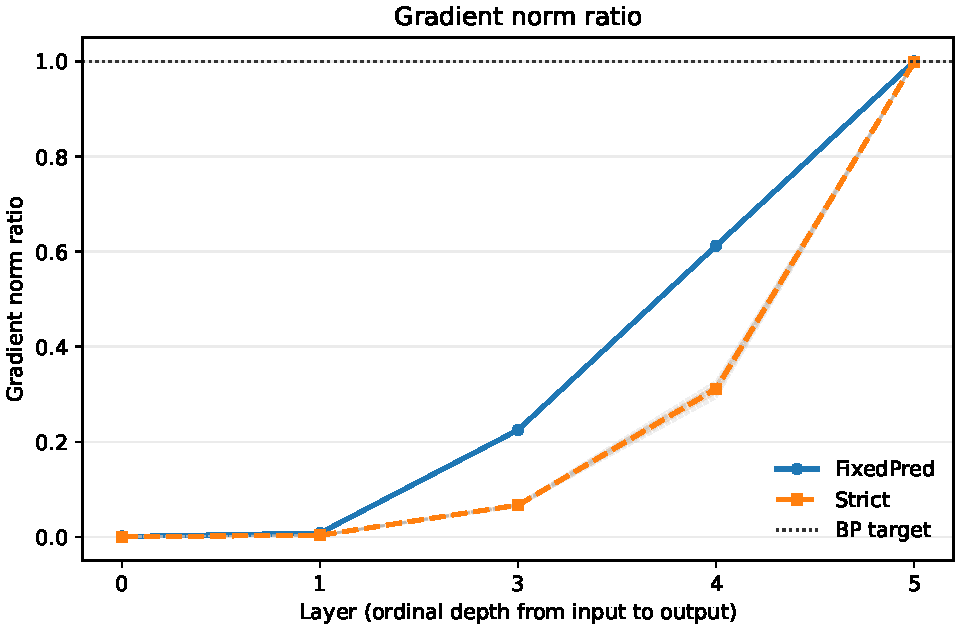
\includegraphics[width=0.82\textwidth]{../results/stage3/layerwise/confirmatory/figures/gradient_norm_ratio_by_depth.pdf}
  \caption{Gradient-norm ratio relative to BP by depth in Stage~3A. The figure is a tracked confirmatory artifact.}
  \label{fig:stage3a-gradient-norm-en}
\end{figure}

\begin{figure}[htbp]
  \centering
  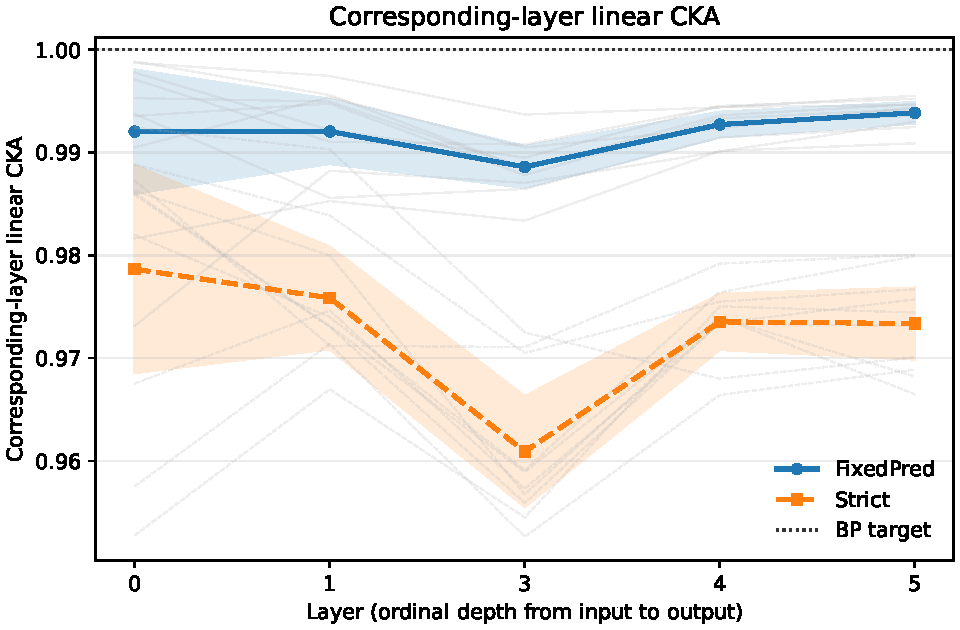
\includegraphics[width=0.82\textwidth]{../results/stage3/layerwise/confirmatory/figures/representation_cka_by_depth.pdf}
  \caption{CKA relative to BP by depth in Stage~3A.}
  \label{fig:stage3a-cka-en}
\end{figure}

Together, Stage~3A supports C02 in a bounded descriptive-comparative sense: FixedPred
shows higher observed similarity to BP than Strict in gradient direction and
representation metrics, but this does not imply matching early-gradient magnitude and
is not interpreted as an unregistered superiority test of FixedPred over Strict.

\section{Stage 3B: Cost Localization and Mechanistic-attribution Tests}
\label{sec:results-stage3b-en}

\input{generated/stage3_results_EN.tex}

B0 localized the principal device-time region to \texttt{state\_inference} for both
methods. Its median share was approximately 71.8\% for FixedPred and 78.8\% for
Strict. In paired configuration-level comparisons, the median Strict/FixedPred device-
time ratio was approximately 2.327 and the peak-allocated-memory ratio 1.328. Median
bytes of saved tensors within \texttt{state\_inference} were approximately twelve
times larger for Strict than FixedPred.

\begin{figure}[htbp]
  \centering
  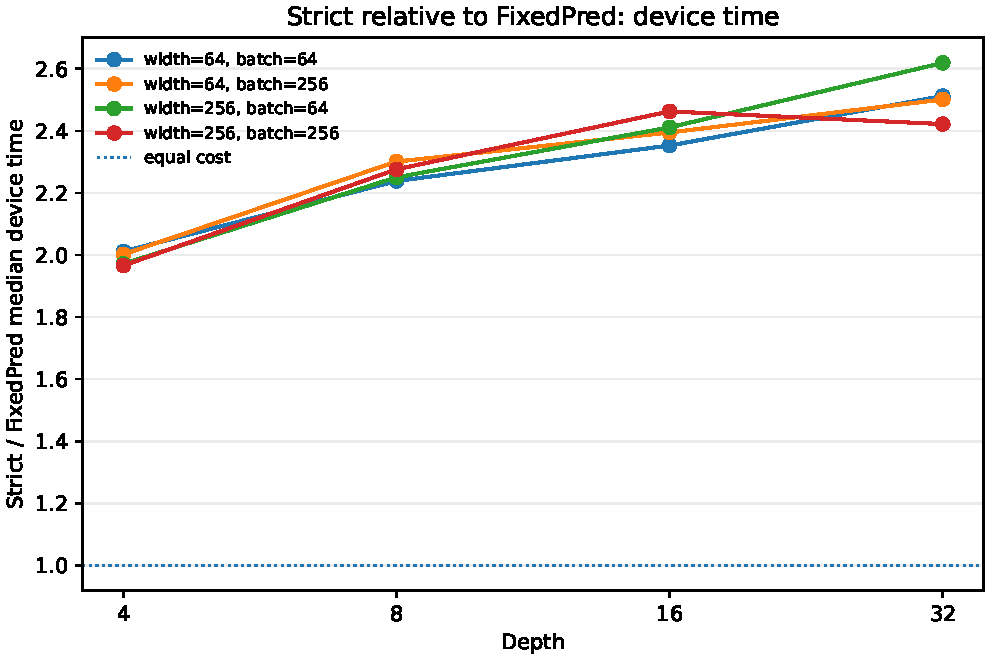
\includegraphics[width=0.82\textwidth]{../results/stage-3/profiling/b0/analysis-v1/paired_device_time_ratio_by_depth.pdf}
  \caption{Paired Strict/FixedPred device-time ratio on the B0 scaling matrix.}
  \label{fig:b0-device-ratio-en}
\end{figure}

C03 (\texttt{supported}) records this B0 localization and observed cost difference.

C04 (\texttt{supported}) records the negative outcome of the first mechanistic
cost-attribution model. SI-MA0 failed COST-MA0: none of 7,500 measured steps satisfied
the registered cost gate. The result was not redefined after later calibration.

C05 (\texttt{supported}) concerns the independent SI-MA1 calibration. CAL-COST-MA1
passed. Across ten model seeds and 180 matched blocks, the observed signed residual was
negative and the upper one-sided 95\% bound remained below the 0.01 threshold. Under
the registered semantics, this is over-closure of the accounting model, not negative
physical operation duration.

C06 (\texttt{supported}) records that both exact candidates passed their equivalence
gates. B1 completed 120/120 registered pairs with no failed pairs or dangerous misses.
B2 completed 120 matched triples and 240 pairwise comparisons, also without failed
pairs. Matched profiling then sealed 288/288 cells and 96 cross-candidate correctness
blocks with no retries.

After matrix freeze, the published descriptive analysis applied the registered
engineering-continuation screen to four B1/B2-by-FixedPred/Strict groups of 16
configurations each. No configuration qualified in any group: every group yielded
0/16, and both B1 and B2 received \texttt{reject\_or\_revise}. Passing EQ-B1 and EQ-B2
therefore did not imply passage of the separate resource-continuation criterion.

This bounded negative engineering result must remain separate from a superiority claim.
The publication receipt permits descriptive reporting but explicitly forbids a
superiority claim. C07 therefore records both completion of the 288-cell surface and
the engineering decision without selecting a ``best'' B1/B2 or establishing universal
non-viability of either computational organization.

\section{QWake-FP C1/C2: Sufficiency, Recognizability, and Economics}
\label{sec:results-qwake-en}

C2 produced a mixed but sharply localized result. Structural reconciliation of the
time surface shows that 108 trajectories yield seven decision epochs
\(t=0,\ldots,6\). The highest-coverage rule among rules with zero observed dangerous
accepts, \texttt{compute\_step >= 5}, accepts exactly two epochs per trajectory: 108
preterminal records at \(t=5\), with one remaining sweep, and 108 terminal-boundary
records at \(t=6\). Because the rule has zero registered dangerous accepts, all 108
accepted step-5 records are preterminal records whose states the post-action reference
assigns to \texttt{EARLY\_ADMISSIBLE}.

Most frozen rules had at least one dangerous accept, but non-zero pre-action
recognizability with zero observed dangerous accepts existed on the calibration
surface: 265 rules had zero dangerous accepts, and 264 of them also had non-zero
coverage. Thus, the first two RQ3 levels---task-relative admissibility of the registered
analytic action and bounded calibration recognizability---receive positive answers.
However, the highest-coverage rule uses only \texttt{compute\_step >= 5}. C08 therefore
establishes a structural temporal boundary equivalent to a fixed prefix on this
surface, not input-content-dependent adaptivity or superiority of PC-CATM features.
This is not a population-risk estimate; independent confirmatory C3 did not open.

\input{generated/qwake_results_EN.tex}

The registered coverage of that rule remains the original C2 quantity: 216/756 records,
approximately 28.57\%, with zero dangerous accepts. It refers to the complete
calibration surface, including the terminal boundary, and is not interpreted as the
fraction of preterminal uses of the analytic action. Under frozen full decision-cost
accounting, aggregate net saving remained negative; indeed, none of the 2,625 rules had
positive aggregate net saving.

Cost decomposition shows approximately 15,096 seconds of aggregate full decision cost
for this rule, compared with approximately 4.98 seconds of registered
\texttt{remaining\_suffix\_ns} over accepted non-dangerous records. Because the
accepted set includes the terminal boundary, this quantity is not interpreted as pure
time of avoidable iterative sweeps. Approximately 99.887\% of full decision cost is
assigned to the observer category. Break-even under the same accounting would require
approximately 99.967\% reduction of the accounted cost. The C2 estimand and cost model
are not recomputed after this structural reconciliation.

The full cost is not interpreted as measured marginal cost of executing
\texttt{compute\_step >= 5}. C2 charged every rule the same frozen per-record decision
cost. C09 is therefore rejected only under that accounting model, whereas C10---the
economic non-viability of a minimal recognizer---remains \emph{untested}.

C08 has status \texttt{supported}, C09 \texttt{rejected}, and C10/C11
\texttt{not\_tested}. Since no eligible rule existed, no C2 rule-freeze receipt was
created and C3 did not open. Absence of confirmatory C3 is therefore a direct
consequence of protocol and the bounded negative C2 result, not a missing run.

\section{Reconciliation with the Research Questions}
\label{sec:results-rq-reconciliation-en}

For RQ1, Stage~1/2 and Stage~3A separate final quality from internal agreement.
Similarity of test metrics does not imply identical gradients, representations, or
runtime. FixedPred preserves gradient direction substantially better than Strict in the
studied domain while retaining strong early-gradient scale suppression.

For RQ2, B0, SI-MA0/1, and B1/B2 progressively narrowed the cost explanation to
\texttt{state\_inference} and testable implementation candidates. The negative SI-MA0
remained an independent result; successful SI-MA1 calibration did not redefine it;
and passage of EQ-B1/EQ-B2 did not imply passage of the later engineering screen: all
four B1/B2-by-FixedPred/Strict groups qualified 0/16 configurations and both candidates
received \texttt{reject\_or\_revise}.

For RQ3, the sealed surface contains preterminal records whose states make the early
action task-admissible: the highest-coverage zero-danger rule accepts 108 such records
at step 5 with one remaining sweep and zero observed dangerous accepts. Its original
registered coverage, 216/756, additionally contains 108 terminal-boundary records and
is not treated as preterminal coverage. Economic benefit under frozen full decision-
cost accounting was not observed. Task-relative admissibility, recognizability, and
economic viability therefore have separate answers; marginal economic viability of a
concrete implementation remains an open question for future work.
